\documentclass[conference]{IEEEtran}
\usepackage[spanish, activeacute]{babel}
\usepackage[utf8]{inputenc}
\usepackage{amsmath, amssymb}
\usepackage{graphicx}
\usepackage{anysize}
\usepackage{hyperref}
\usepackage{caption}
\usepackage[table]{xcolor}
\usepackage{booktabs}

\usepackage{color}
\newcommand{\todo}{\textcolor{red}{TO DO:}\textcolor{blue}}

\title{Primeros pasos del Observatorio Virtual Chileno}
\author{
\IEEEauthorblockN{
	Mauricio Solar \IEEEauthorrefmark{1}, Jonathan Antognini \IEEEauthorrefmark{1}, Marcelo Mendoza \IEEEauthorrefmark{1}, Jose Marroquín \IEEEauthorrefmark{1}, Cristián Maureira \IEEEauthorrefmark{1} \\
	Jorge Ibsen \IEEEauthorrefmark{2}, Lars Nyman \IEEEauthorrefmark{2}, 
	Eduardo Vera \IEEEauthorrefmark{3}, Diego Mardones \IEEEauthorrefmark{3}, Guillermo Cabrera \IEEEauthorrefmark{3},\\
	Paola Arellano \IEEEauthorrefmark{4},
	Karim Pichara \IEEEauthorrefmark{5}, Nelson Padilla \IEEEauthorrefmark{5},
	Ricardo Contreras \IEEEauthorrefmark{6}, \\ Neil Nagar \IEEEauthorrefmark{6},
	Victor Parada \IEEEauthorrefmark{7}.
}

\\

\IEEEauthorblockA{\IEEEauthorrefmark{1} Universidad Técnica Federico Santa María, Valparaiso, Chile}
\IEEEauthorblockA{\IEEEauthorrefmark{2} Atacama Large Millimeter/submillimeter Array, San Pedro de Atacama, Chile}		
\IEEEauthorblockA{\IEEEauthorrefmark{3} Universidad de Chile, Santiago, Chile}							
\IEEEauthorblockA{\IEEEauthorrefmark{4} Red Universitaria Nacional, Santiago, Chile}						
\IEEEauthorblockA{\IEEEauthorrefmark{5} Universidad Católica de Chile, Santiago, Chile}					
\IEEEauthorblockA{\IEEEauthorrefmark{6} Universidad de Concepción, Concepción, Chile}					
\IEEEauthorblockA{\IEEEauthorrefmark{7} Universidad de Santiago de Chile, Santiago, Chile}
}

\begin{document}

\maketitle

\begin{abstract}
Este documento muestra la distribución de observatorios virtuales a lo largo del
mundo, y como sería la distribución ante la eventual inclusión de Chile.
Por otro lado se presenta el concepto Observatorio Virtual, las necesidades
por las cuales surge este propósito, y los protocolos y estándares que desarrollan en
conjunto. Además se mostrará la arquitectura por niveles y capas que componen
una plataforma de este tipo y los primeros pasos de Chilean Virtual Observatory.
\end{abstract}

\begin{IEEEkeywords}
	IVOA, Chivo, Virtual Observatory.
\end{IEEEkeywords}

\section{Introducción}

Las provilegiadas condiciones atmosféricas hacen de Chile uno de los lugares
más propicios para la realización de investigaciones científicas en astronomía.
Organizaciones astronómicas como el Observatorio Europeo Austral (ESO por sus
siglas en inglés) han elegido asentar sus enormes telescopios en este país para 
llevar a cabo sus descubrimientos\footnote{Acerca de ESO. (s.f.). En
\textit{ESO}. \url{http://www.eso.org/public/chile/about-eso.html}}. 

Existen más de una docena de instalaciones astronómicas de gran envergadura a
lo largo de nuestro territorio nacional \cite{observatorios_chile}, como por
ejemplo ``Atacama Large Milimeter/submilimeter Array'' (ALMA), ``Very Large
Telescope'' (VLT), y en los próximos ``European Extremely Large Telescope''
(E-ELT), con el cual se estima que el 60\% de la observación astronómica
mundial se realice en Chile.  Una de las condiciones que se establecen a nivel
país, es que el 10\% del tiempo de observación pertenece a la comunidad
astronómica chilena. Estos generan datos a gran escala, justificando a nivel
país, el desarrollo de una plataforma astroinformática para su administración y
análisis inteligente.

El Observatorio Virtual (VO por sus siglas en inglés) es una iniciativa
internacional que permite el acceso a archivos astronómicos y centros de datos
a astrónomos y personas comunes a través de Internet. Con la estandarización de
métodos e información es posible estudiar los registros astronómicos sin
requerimientos físicos de instrumentos y locación.

La International Virtual Observatory Alliance (IVOA) fue creada para
``facilitar la coordinación internacional y colaboración necesaria para el
desarrollo y distribución de herramientas, sistemas y estructuras
organizacionales necesarias para permitir la utilización internacional de
archivos astronómicos como un observatorio virtual integrado e 
interoperable\footnote{Traducido de \url{http://www.ivoa.net/about/what-is-ivoa.html}}.
Actualmente, IVOA está compuesta por 19 proyectos\footnote{En el sitio web oficial en la
sección \textbf{What is the IVOA} \textit{``the IVOA now comprises 17 VO
projects''}, pero en \textbf{Members Organizations} aparecen 19 miembros
listados.} de América, Asia, Europa y Oceanía; sus miembros se reunen
dos veces cada año en \textbf{Interoperability Workshops} para entablar
discusiones cara-a-cara y resolver preguntas técnicas.

Actualmente una iniciativa liderada por la UTFSM propone
desarrollar una plataforma astro-informática para la administración y análisis
inteligente de datos a gran escala basados en los estándares de IVOA.  Por lo
anterior, este documento tiene como objetivo:

\begin{itemize}
	\item Dar a conocer la distribución de los VO's en el mundo.
	\item Explicar el concepto de VO.
	\item Explicar la arquitectura a grandes rasgos de un
		VO.
	\item Presentar los primeros pasos para llevar a cabo el
		Chilean Virtual Observatory (ChiVO).
	\item Conclusiones y trabajo a futuro.
\end{itemize}

\section{Distribución de los VO's en el mundo}
\subsection{IVOA}

Desde el año 2002, proyectos de VO's comenzaron a integrar
la Alianza Internacional Observatorio Virtual bajo el \textbf{Guidelines
for Participation\footnote{La documentación se puede
encontrar en \url{http://www.ivoa.net/documents/latest/IVOAParticipation.html}}}.

Estos fueron fundados bajo programas privados y gubernamentales nacionales e
internacionales en colaboración con centro de estudios científicos,
universidades y otros. Quienes integran este proyecto, el Observatorio Virtual, 
comparten conocimientos entre ellos y la comunidad de modo estandarizado. Son 
ellos mismos quienes desarrollan estos estándares para el intercambio de 
información e interoperabilidad.

El cuadro \ref{table:integrantes} muestra los miembros de IVOA hasta mayo de
2013
%\footnote{\todo{Se supone que lo que dices aquí se aplica a todo el paper,
%y está de más, pues el comité que revise dira si es todo verídico o no}
%En este documento, toda la información recuperada del sitio
%web oficial de IVOA es considerada oficial y verídica.}.
%\todo{Agregar los links de la tabla~\ref{table:integrantes} como referencias, usar entrada @Misc. ver .bib}

\begin{table}[h!t]
	\centering
	\begin{tabular}{l} \hline
		%\hline
		\textbf{Proyecto} \\\hline
			Argentina Virtual Observatory\cite{arg} \\
			Armenian Virtual Observatory\cite{arm}\\
			AstroGrid\cite{astrogrid}\\
			Australian Virtual Observatory\cite{aus}\\
			Brazilian Virtual Observatory\cite{bra}\\
			Canadian Virtual Observatory\cite{can}\\
			Chinese Virtual Observatory\cite{china}\\
			European Space Agency\cite{esa}\\
			European Virtual Observatory\cite{euro}\\
			German Astrophysical Virtual Observatory\cite{ger}\\
			Hungarian Virtual Observatory\cite{hun}\\
			Italian Virtual Observatory\cite{ita}\\
			Japanese Virtual Observatory\cite{jap}\\
			Observatorie Virtual France\cite{fra}\\
			Russian Virtual Observatory\cite{rus}\\
			Spanish Virtual Observatory\cite{spa}\\
			Ukranian Virtual Observatory\cite{ukr}\\
			Virtual Astronomical Observatory\cite{usa}\\
			Virtual Observatory India\cite{ind}\\
            \hline
	\end{tabular}
	\caption{Integrantes de IVOA}
	\label{table:integrantes}
\end{table}

Casi la mitad de los observatorios virtuales de IVOA están en Europa: 9 del
total; 1 pertenece a Oceanía, 4 a América y 5 de ellos a Asia \footnote{Como la
mayor parte de Rusia está en territorio Asiático, es considerado como uno de
los VO's de ese contintente.} La figura 1 muestra la distribución de los
miembros de IVOA por continente.
	\begin{figure}[h!t]
		\begin{center}
			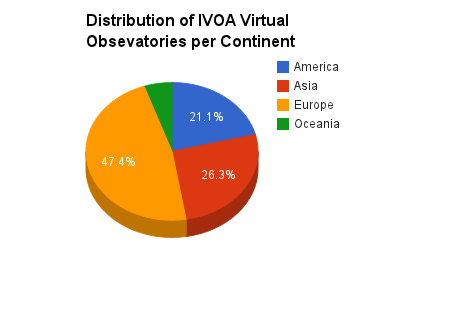
\includegraphics[width=0.5\textwidth]{img/ivoa_vos_distribution.png}
			\caption{Distribución por continente de IVOA.}
		\end{center}
	\end{figure}

Si Chile se convirtiera en miembro de IVOA, la distribución de los miembros
por continentes sería la que se muestra en la figura 2.
	\begin{figure}[h!t]
		\begin{center}
			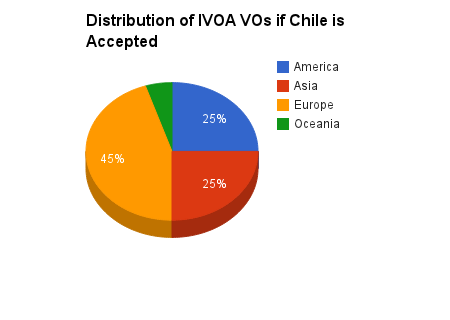
\includegraphics[width=0.5\textwidth]{img/if_chile_is_accepted.png}
			\caption{International Virtual Observatory Alliance Distribución por continente incluyendo a Chile.}
		\end{center}
	\end{figure}

Sin considerar el estado de los proyectos internos de los VO's, 
la membresía de Chile contribuiría a que América, llegue a la misma
cantidad en número de VO's que Asia. Por otra parte, este
hecho sería muy significativo, ya que un gran número de centros astronómicos
como los observatorios se instalan en este país. Por ahora, se pretende
trabajar con datos del proyecto ALMA.

%\section{Lista of los observatorios virtuales de IVOA y sus proyectos}
\subsection{América}
\subsubsection{Brazilian Virtual Observatory (BRAVO)}
BRAVO, es una iniciativa que empezó formalmente por medio de una declaración de
intenciones de participar en agosto del 2006, por los representantes legales de
seis institutos de investigación brazileños, más la sociedad astronómica de
Brazil. Algunos proyectos: 
	\begin{itemize}
		\item BRAVO @Instituto de Astronomía, Geofísica y Ciencias Atmosféricas:
			\begin{itemize}
				\item StarLight: es un mirror del webservice Starlight alojado en \url{www.starlight.ufsc.br}
				\item GALExtin: es una herramienta que permite determinar la extinción a lo largo de una línea de visión.
				\item ZPhot: herramienta de redshifts fotométricos.
				\item RedSpec: herramienta de reddening y reddening.
				\item Be Atlas: esta herramienta pone a disposición de la comunidad 70.000 espectros sintéticos de Be stars.
			\end{itemize}
		\item BRAVO @Instituto Nacional de Investigación Espacial de Brasil: Generar inversiones en tecnología de información en infraestuctura computacinal, Grid de datos, Procesamiento de datos y 
				Minería de datos.
		%\begin{itemize}
		%	\item Descripción: generate investment in information technology on Computational Infraestructure, Date Grid, Data Processing and Data Mining.
		%\end{itemize}
		\item BRAVO @Laboratorio Nacinal de Astrofísica: creando un observatorio virtual dedicado al data del Southern Astrophysical Research Telescope (SOAR), para los astrónomos brasileños.
		%\begin{itemize}
		%	\item Descripción: Making of a virtual observatory dedicated to Southern Astrophysical Research Telescope (SOAR) data from Brazilian astronomers.
		%\end{itemize}
		\item BRAVO @Universidad Federal de Santa Catarina: investigando en la síntesis espectral de potencia como un medio para estimar las propiedades físicas de las galaxias.
		%\begin{itemize}
		%	\item Descripción: researching of the of the power spectral synthesis as a mean to estimate the physical properties of the galaxies.
		%\end{itemize}
		\item Cyclotron Emission of Polars (CYCLOPS): han desarrollado un nuevo código, para modelar la emisión óptica de estos sistemas, incluyendo los cuatros parámetros de Stokes.
	\end{itemize}
\subsubsection{Canadian Virtual Observatory (CVO)}
	\begin{itemize}
		\item Proyectos
		\begin{itemize}
			\item Data Sharing (VOSpace 2.0)
			\begin{itemize}
				\item Descripción: a service which allows users to share files and collaborate with team members.  
			\end{itemize}
			\item Table Access Protocol (TAP-1.0)
			\begin{itemize}
				\item Descripción: a service which allows the access to all the data described by the Common Archive Observation Model (CAOM) in use at the CADC and tables from other projects.
			\end{itemize}
			\item Observation Model Core Components (ObsCore-1.0)
			\begin{itemize}
				\item Descripción: a model which implements a standard view for \textbf{Table Access Protocol (TAP-1.0)}.
			\end{itemize}
			\item Simple Image Access (SIA-1.0)
			\begin{itemize}
				\item Descripción: a SIA-1.0 compliant query service for easy access to calibrated images from most our data collections.
			\end{itemize}
		\end{itemize}
	\end{itemize}

\subsubsection{Nuevo Observatorio Virtual Argentino (NOVA)}
	\begin{itemize}
		\item Fundadores: Observatorio Astronómico de Córdova (OAC),
			Facultad de Ciencias Astronómicas y Geofísicas de La Plata/Universidad de
			Nacional de la Plata (FCAGLP/UNLP), Instituto de Astrofísica de La Plata
			(IALP), Instituto Argentino de Radioastronomía (IAR), Instituto de Astronomía y
			Física del Espacio (IAFE), Instituto de Ciencias Astronómicas, de la Tierra y
			del Espacio (ICAFE), Instituto de Astronomía Teórica y Experimental (IATE),
			Complejo Astronómico El Leoncito (CASLEO).
		\item Comienzo: January, 2009
		\item Proyectos
		\begin{itemize}
			\item NOVA@CASLEO
			\begin{itemize}
				\item Estado: active.
				\item Descripción: not obtained for now. Not available at NOVA's website or similar.
			\end{itemize}
			\item NOVA@IAFE
			\begin{itemize}
				\item Estado: unknown.
				\item Descripción: building a database for the spectroscopic observations available at ICATE.
				\item Outstanding: until 1987, the database was stored in photographic plates. After that year, the information was stored in CDs and DVDs.
			\end{itemize}
			\item NOVA@ICATE
			\begin{itemize}
				\item Estado: unknown.
				\item Descripción: building a database for the spectroscopic observations available at ICATE.
				\item Outstanding: until 1987, the database was stored in photographic plates.
					After that year, the information was stored in CDs and DVDs.
			\end{itemize}
			\item NOVA@OAC
			\begin{itemize}
				\item Estado: active.
				\item Descripción: not obtained for now. Not available at NOVA's website or similar.
			\end{itemize}
			\item NOVA@FCAGLP, NOVA@IALP, NOVA@IAR, NOVA@IATE are referred in the website but without status and description.
		\end{itemize}
	\end{itemize}

\subsubsection{US Virtual Astronomical Observatory (VAO)}
	\begin{itemize}
		\item Fundadores: NSF, NASA.
		\item Proyectos
		\begin{itemize}
			\item Data Discovery Tool
			\begin{itemize}
				\item Descripción: 
			\end{itemize}
			\item Iris: SED Analysis Tool
			\begin{itemize}
				\item Descripción: 
			\end{itemize}
			\item Cross-Comparision Tool
			\begin{itemize}
				\item Descripción: 
			\end{itemize}
			\item Time Series Search Tool
			\begin{itemize}
				\item Descripción: 
			\end{itemize}
		\end{itemize}
	\end{itemize}

\subsection{Europe}
\subsubsection{Armenian Virtual Observatory}
	\begin{itemize}
		\item Proyectos
	\end{itemize}

\subsubsection{Hungarian Virtual Observatory (HVO)}
	\begin{itemize}
		\item Proyectos
	\end{itemize}

\subsubsection{AstroGrid}
	\begin{itemize}
		\item Comienzo: 2001
		\item Fundadores: PPARC, STFC
		\item Proyectos
		\begin{itemize}
			\item VODesktop
			\begin{itemize}
				\item Descripción: an analysis tools wich allows limit the choice of resources through specific data saving.
			\end{itemize}
			\item Astro Runtime (AR)
			\begin{itemize}
				\item Descripción: an API implemented in JAVA wich facilitates the access to the \textbf{VODesktop} services from any programming language.
			\end{itemize}
		\end{itemize}
	\end{itemize}

\subsubsection{European Space Agency Virtual Observatory (ESA-VO)}
	\begin{itemize}
		\item Proyectos
	\end{itemize}

\subsubsection{European Virtual Observatory (EURO-VO)}
	\begin{itemize}
		\item
	\end{itemize}

\subsubsection{German Astrophysical Virtual Observatory (GAVO)}
	\begin{itemize}
		\item Proyectos
		\begin{itemize}
			\item GAVO Data Center
			\begin{itemize}
				\item Descripción: A growing collection of data and services provided on behalf of third parties. Some of the GAVO services are also available on http://dc.zah.uni-heidelberg.de/
			\end{itemize}
			\item MPA Simulations access
			\begin{itemize}
				\item Descripción: a web service for querying the results of the Millennium simulation using SQL.
			\end{itemize}
			\item MultiDark Database
			\begin{itemize}
				\item Descripción: a service wich gives access to data from MultiDark and Bolshoi simulations using SQL queries. It based on the Millennium Web Application.
			\end{itemize}
			\item RAVE archive search
				\begin{itemize}
				\item Descripción: an access to a growing archive of radial velocities for more than 400 000 stars.
			\end{itemize}
			\item TheoSSA
				\begin{itemize}
				\item Descripción: a service for providing spectral energy distributions based on model atmosphere calculations.
			\end{itemize}
		\end{itemize}
	\end{itemize}

\subsubsection{Observatoire Virtuel France (VO-France)}
	\begin{itemize}
		\item Proyectos
	\end{itemize}

\subsubsection{Spanish Virtual Observatory (SVO)}
	\begin{itemize}
		\item Proyectos
		\begin{itemize}
			\item VOSA
			\begin{itemize}
				\item Descripción: 
			\end{itemize}
			\item VOSED
			\begin{itemize}
				\item Descripción: 
			\end{itemize}
			\item TESELA
			\begin{itemize}
				\item Descripción: 
			\end{itemize}
			\item Filter Profile Service
			\begin{itemize}
				\item Descripción: 
			\end{itemize}
		\end{itemize}
	\end{itemize}

\subsubsection{Italian Virtual Observatory (VObs.it)}
	\begin{itemize}
		\item Comienzo: 2005
		\item Fundadores: INAF
		\item Proyectos
		\begin{itemize}
			\item SIAP
			\begin{itemize}
				\item Descripción: 
			\end{itemize}
			\item SSAP
			\begin{itemize}
				\item Descripción: 
			\end{itemize}
			\item CONE SEARCH
			\begin{itemize}
				\item Descripción: 
			\end{itemize}
			\item SKYNODE
			\begin{itemize}
				\item Descripción: 
			\end{itemize}
		\end{itemize}
	\end{itemize}

\subsection{Asia}
\subsubsection{Chinese Virtual Observatory}
	\begin{itemize}
		\item Proyectos
	\end{itemize}

\subsubsection{Japanese Virtual Observatory}
	\begin{itemize}
		\item Proyectos
	\end{itemize}

\subsubsection{Russian Virtual Observatory}
	\begin{itemize}
		\item Proyectos
	\end{itemize}

\subsubsection{Virtual Observatory India}
	\begin{itemize}
		\item Fundadores: Persistent Systems Ltd.
		\item Colaboradores: Inter-University Centre for Astronomy and Astrophysics (IUCAA).
		\item Soporte: Ministry of Communication and Information Technology, Government of India.
		\item Comienzo: January, 2009
		\item Proyectos
		\begin{itemize}
			\item VOIPortal
			\item Mosaic Service
			\item PyMorph Service
			\item VOPlot
			\item VOMegaPlot (Client-Server Version)
			\item AstroStat
			\item VOCat
			\item VOPlatform
			\item VOConvert (ConVOT)
			\item Android Cosmological Calculator
			\item Android Name Resolver
			\item CSharpFITS Package
			\item VOTable JAVA Streaming Writer
			\item C++ parser for VOTable
			\item Fits Manager
			\item HCT Data Archival Sys
		\end{itemize} 	
	\end{itemize}


\section{Concepto de Observatorio Virtual}

\emph{``En la actualidad se está generando una ingente cantidad de datos
provenientes de un número creciente de instrumentos astronómicos con cada vez
mejor resolución, lo que está multiplicando las neceisdades de almacenamiento''.}
\footnote{El Observatorio virtual, Por Juan de Dios Santander (IAA-CSIC)}

Esta frase refleja problemáticas que se presentan a la actualidad, pero desde
otro punto de vista también son oportunidades de cubrir ciertas necesidades.
Algunas necesidades son:
%\emph{Algunas de estas son}:

%\todo{Resaltar la palabra o palabras antes del ``:'', con negrita o emph}
\begin{itemize}
	\item Facilidad de acceso: en el mundo existen distintos instrumentos
		astronómicos, los cuales generan volúmenes de datos a gran escala,
		por lo que es necesario unificar la forma en que se publica esta información
		de tal modo que no sea difícil encontrar los detalles requeridos.
	\item Información relativa a los datos: cuando se habla de datos en
		astronomía es necesario entender el contexto en el cual se desenvuelven.
		Los datos en astronomía pueden ser listas de números, matrices de números
		(píxeles de una imagen por ejemplo) o arreglos de más de dos dimensiones.
		Si una persona, independiente que sea astrónomo, busca cierto
		conjunto de datos, necesita saber cómo hacerlo, es decir,
		qué parámetros, campos, descripciones poseen los mismos.
		Respecto a esto, en astronomía se han generado distintos formatos
		de datos astronómicos, por ejemplo, ``Flexible Image Transport System''\cite{fits_definition}
		(FITS).	La necesidad en cuestión es que los datos elaborados por un grupo de
		investigación pueda ser utilizado por cualquier otro.
	\item Procesamiento de datos: algunos datos, al poseer volúmenes grandes,
		necesitan ciertas capacidades de almacenamiento \cite{archive_tsunami} y cómputo \cite{data_hpc}.
		Por lo que los VO's ayudan a reducir la transferencia de información.
	\item Minería de datos: los datos son una fuente de valor importante para los
		astrónomos y científicos en general, por lo que constantemente se hacen esfuerzos
		en enriquecerlos. La manera en que se hace este proceso, es usando técnicas de 
		minería de datos \cite{vo_data_mining}, \emph{para}: reconocimiento de patrones, priorización
		de información, clasificación de estrellas, representatividad de datos, etc.;
		Por lo que es necesario proveer algoritmos que cumplan dicha labor.
		%\todo{Me esperaba mas información
		%    acá, debido aque el data mining o creacion de algoritmos que hagan tareas
		%    automáticas es y sera nuestro fuerte}
	\item Notificación y registro de servicios y datos nuevos: los datos
		disponibles estén permanentemente actualizados.
\end{itemize}

%Las necesidades que surgieron desde la comunidad astronómica y el
%aprovechamiento de las oportunidades que emergirían de las mismas, incentivó
%a la creación de una alianza internacional: la IVOA.
Al ir apareciendo distintas necesidades en la comunidad astronómica, se creó una alianza internacional entre 
distintos centros de investigación para aprovechar las oportunidades que fueron
apareciendo. Con esto nació IVOA.

\subsection{Protocolos y estándares IVOA}

IVOA fue formada en Junio del 2002.  \emph{Su misión es facilitar la
coordinación y colaboración necesaria para facilitar el acceso global e
integrado a los datos recogidos por los observatorios astronómicos
internacionales}.

Su principal función en la actualidad es crear, versionar y mantener informada
a la comunidad acerca de los protocolos y estándares \cite{ivoa_documents} a
usar.  Eso lo llevan a cabo mediante los Working Groups. Ellos preparan
documentos disponibles para toda la comunidad, los cuales describen distintas
funcionalidades, arquitecturas, normas, etc. para un observatorio virtual.
El diagrama de cómo se crean estos estándares está representado
en la figura~\ref{fig:creacionestandares}.
\begin{figure}[h!t]
        \centering
         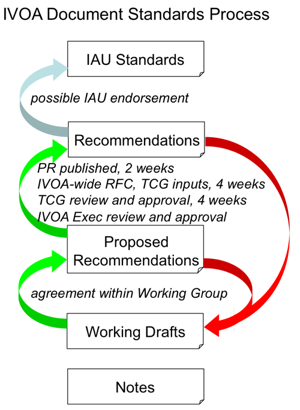
\includegraphics[width=0.45\textwidth]{img/diagrama_proceso.png}
         \caption{Creación de Estándares IVOA}
        \label{fig:creacionestandares}
\end{figure}

%\todo{poner esto como itemize, enumerate, o description, así se ve super feo}
Los \textbf{Working Groups}: se encargan de elaborar
o versionar los estándares que se subdividen en \emph{áreas técnicas}: \\
\begin{itemize}
	\item \textbf{Aplicaciones}: se encarga de las herramientas de software que los
		astrónomos utilizan en su labor para acceder a los datos y servicios. \\
	\item \textbf{Capa de acceso a los datos}: definen y formulan estándares para el
		acceso remoto a los datos. Se orientan a funciones para clientes y publishers. \\
	\item \textbf{Modelamiento de datos}: proporcionan un marco para la descripción de
		los metadatos asociados a los datos observados (o simulados). Se orientan a
		relaciones lógicas entre esos metadatos y el modo en que los astrónomos quieren examinar. \\
	\item \textbf{Grid y servicios web}: definen el uso de tecnología de redes y
		servicios de Internet dentro del contexto de VO. \\
	\item \textbf{Registro de recursos}: define la estructura y la interfaz de un \textit{IVOA
		Registry}. Permite a los astrónomos localizar y hacer uso de recursos de VO. \\
	\item \textbf{Semánticas}: exploran el significado o las interpretaciones de palabras o frases,
		o de otro tipo de lenguaje en el contexto de astronomía, como por ejemplo, ontologías. \\
	\item \textbf{Eventos VO}: define el contenido y el significado de un paquete de información
		acerca de un evento celestial transitorio como el paso de un cometa, entre otros. \\
\end{itemize}

\section{Arquitectura de un Observatorio Virtual}

El VO's es un framework que ayuda a resolver distintos
problemas que enfrenta la comunidad astronómica a lo largo del mundo.  Uno de
los problemas está relacionado al acceso a los datos, por lo que en IVOA
diseñaron tecnologías y estándares formalmente definidos, que permitan el de
acceso unificado y transparente a distintos servidores con datos astronómicos.

El beneficio que conlleva es considerable, ya que estos
estándares, protocolos, tecnologías y arquitectura, ayudan a la comunidad al
proceso de creación de servicios, portales web, aplicaciones de escritorio,
etc. Todo visto del punto de vista de ingeniería de software.

\subsection{Arquitectura VO por Nivel}
%\todo{Las figuras se ven super mal en chico, quizás podrías ponerlas a doble
%columna}

IVOA dentro de sus documentos presenta distintos niveles de arquitectura
\cite{ivoa_arch}, con el objetivo de ir aclarando incrementalmente las
funcionalidades (basadas en necesidades) que requiere un VO.

\textbf{Arquitectura Nivel 0} %~\ref{fig:nivel0}\\


La arquitectura más básica que aclara el concepto de VO, se compone por 3
capas:

\begin{enumerate}
    \item Capa de recursos:
          compilado de datos astronómicos provenientes de distintos instrumentos.
    \item Capa de usuarios:
          investigadores que buscan consumir datos.
    \item Capa intermedia:
          es la capa que permite conectar las dos
          capas anteriores de manera transparente para los investigadores.
          Esta interacción se puede llevar a cabo buscando u obteniendo datos.
\end{enumerate}

\begin{figure*}[h!t]
    \centering
    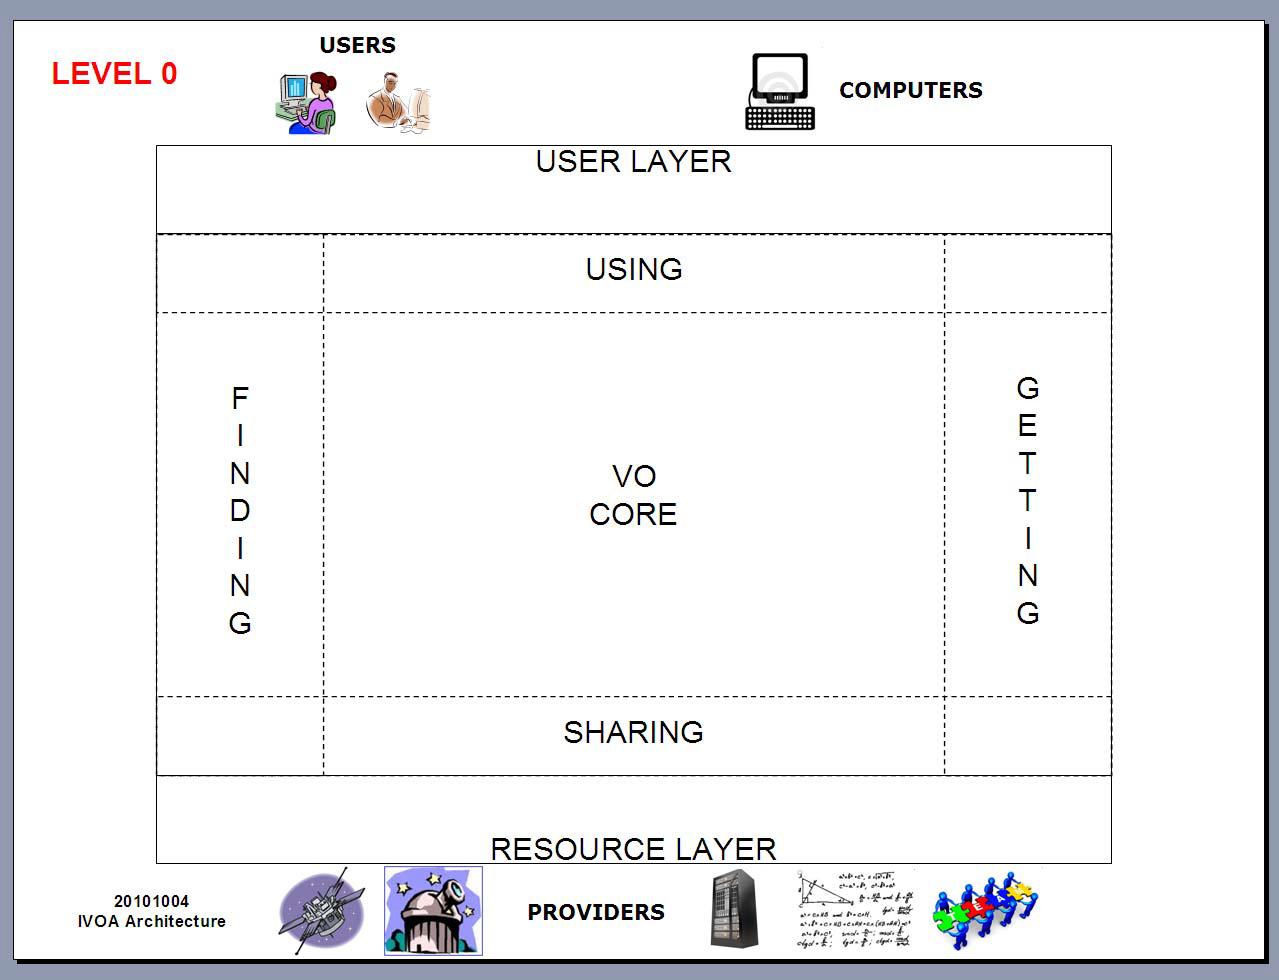
\includegraphics[width=0.7\textwidth]{img/arquitectura_0.png}
    \caption{Arquitectura Nivel 0}
    \label{fig:nivel0}
\end{figure*}

\textbf{Arquitectura Nivel 1}%~\ref{fig:nivel1}


La arquitectura nivel 1 mantiene la misma cantidad de capa pero se especifica:
\begin{enumerate}
    \item Capa de recursos:
          está compuesto de colección de datos y provenientes de distintos
          servidores.
    \item Capa de usuarios:
          un consumidor puede querer acceder a los datos desde un navegador,
          escritorio, o mediante un script.
    \item Capa intermedia:
          crea un framework para compartir los datos, compuesto por VOQL,
          Data Models, Semantics, Formats.
\end{enumerate}

\begin{figure*}[h!t]
    \centering
    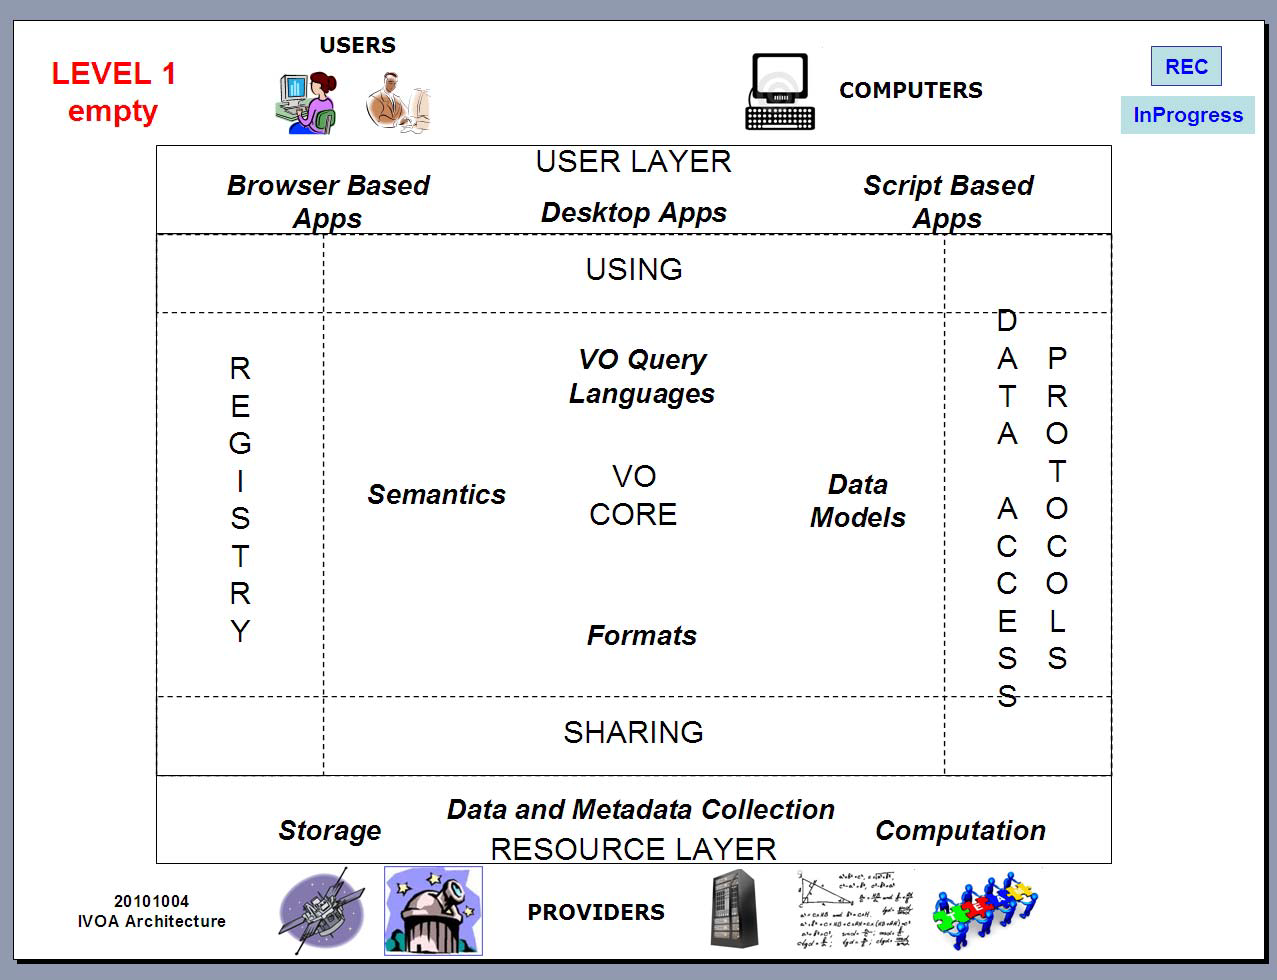
\includegraphics[width=0.7\textwidth]{img/arquitectura_1.png}
    \caption{Arquitectura Nivel 1}
    \label{fig:nivel1}
\end{figure*}

\textbf{Arquitectura Nivel 2}%~\ref{fig:nivel2}


La arquitectura nivel 2 es lo que se entiende por un VO regido por estándares
y protocoloes de IVOA.
La idea de esta figura es seccionar cada estándar relacionándolo específicamente
a la capa a la cual pertenece.

\begin{figure*}[h!t]
    \centering
    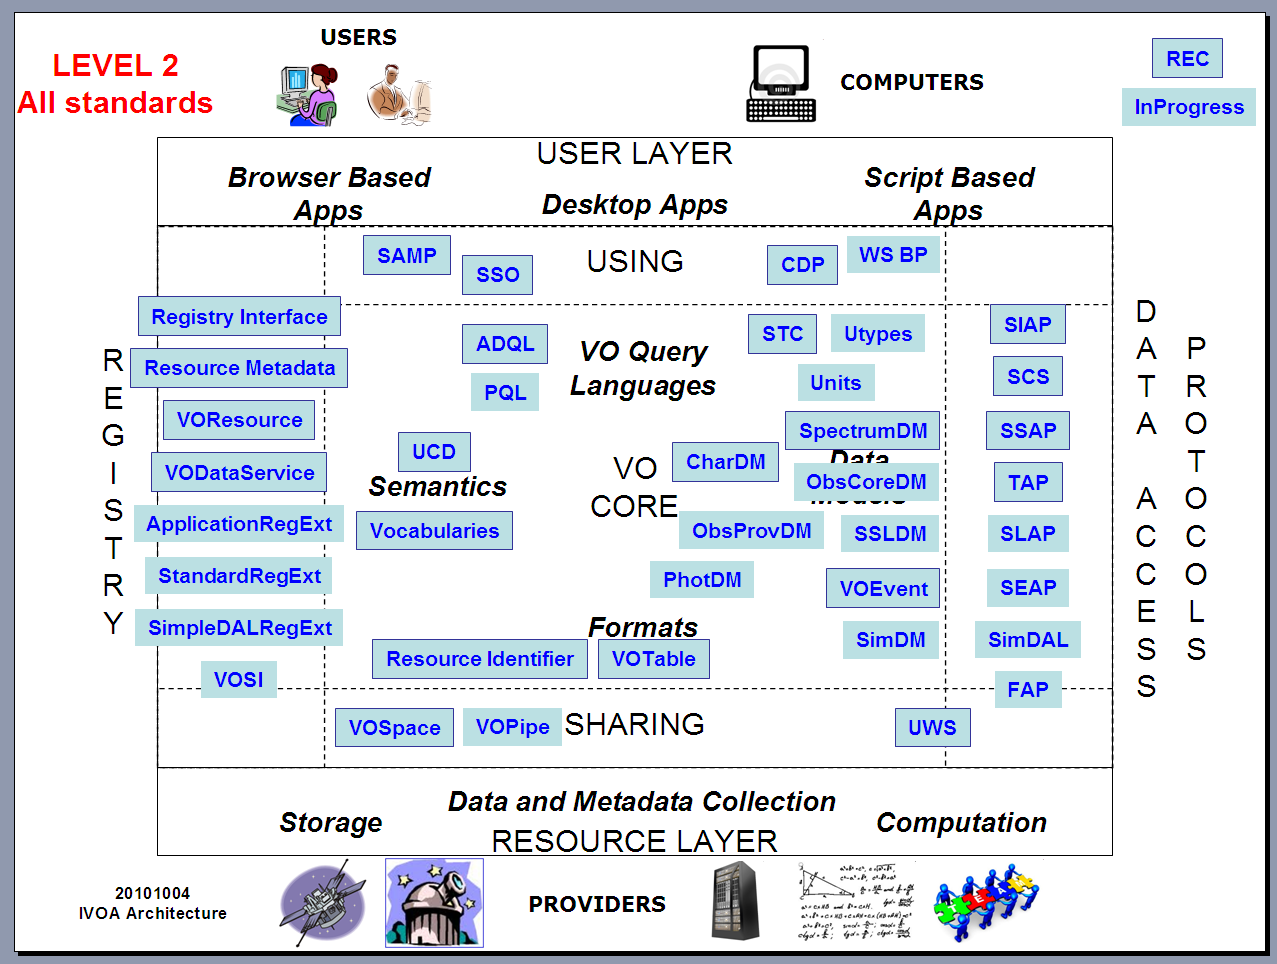
\includegraphics[width=0.7\textwidth]{img/arquitectura_2.png}
    \caption{Arquitectura Nivel 2}
    \label{fig:nivel2}
\end{figure*}

\section{Primeros pasos del Chilean Virtual Observatory}

En el Chilean Virtual Observatory (ChiVO), se han generado instancias y colaboraciones
para llevar a cabo este ambicioso proyecto. En estas, se han clarificado las
posibles limitaciones y necesidades que tendrá la comunidad astronómica en
el mediano plazo con las cuales se han planteado objetivos del sistema. Esta
sección abordará los objetivos del sistema y la iniciativa que está desarrollando ChiVO.

\subsection{Objetivos del sistema}

Los volúmenes de datos a gran escala que generan y generarán los observatorios
astronómicos actuales y futuros en Chile, han suscitado nuevas necesidades que
permiten el desarrollo de nuevas herramientas y técnicas de análisis de datos.

Para tener una idea general de la cantidad de datos que requerirán ser
clasificados y procesados, se puede tomar en cuenta el proyecto ALMA,
inaugurado en marzo del 2013, en el cual se estima que serán generados más de 1
TB de datos diarios en su máxima capacidad operativa.
%en el cual cuando se encuentre completamente operativo
%(con todo su conjunto de antenas), se generarán más de 1 TB de datos por día de
%observación.

La manipulación de altos volúmenes de datos generan complicaciones en diversos
aspectos:
%\begin{itemize}
	%\item Almacenamiento, es necesario tener un centro de procesamiento de datos con
	\textbf{Almacenamiento}, es necesario tener un centro de procesamiento de datos con
		la capacidad de almacenamiento suficiente y acorde a las necesidades de consumo
		de dichos datos, sin dejar de lado el espacio físico que dichos equipos
		necesitarán y la arquitectura detrás del almacenamiento en sí. \\
	\textbf{Acceso}, se deben establecer mecánicas y normativas de accesos para
		cualquier persona, ya sean astrónomos o no, lo cual requiere de un sistema que
                permita acceder a él desde cualquier lugar. En este proyecto
		se ha decidido por sistema web, ya que es un mecanismo adecuado para suplir la
                presente necesidad. \\
	\textbf{Procesamiento}, el procesamiento de datos es un área particular de la
		informática, la cual conlleva a entender tanto la naturaleza como la estructura
		de los datos como también las herramientas y técnicas que se pueden utilizar
		para llevarlo a cabo. Al tener grandes volúmenes de datos, el procesamiento a
		realizar, ya sean correcciones, calibraciones, análisis, etc., exigen más tiempo
		del habitual y por supuesto que más recursos computacionales, elementos que un
		usuario no posee. Es por lo anterior que un cluster computacional puede ser una
		herramienta útil para realizar esta labor. \\
                %Por lo que un cluster computacional, puede ser una herramienta útil para
                %facilitar esta labor.
%\end{itemize}

Los anteriormente detallado pertenece a las motivaciones principales
por las cuales actualmente en Chile se está desarrollando un proyecto que
busca crear una plataforma de procesamiento de datos de gran escala, el cual
compromete como uno de sus entregables un Observatorio Virtual del que se
espera que garantice rapidez y eficiencia tanto al acceso de información
existente y servicios astronómicos como en el análisis de dicha información.

\subsection{Iniciativa que lo desarrolla}
Actualmente se está desarrollando el proyecto titulado ``Desarrollo de una
plataforma astroinformática para la administración y análisis de datos de gran
escala'', financiado con fondos gubernamentales (FONDEF D11I1060) con duración
de 28 meses en el cual participan las siguientes instituciones:
\begin{itemize}
	\item Atacama Large Milimeter/submilimeter Array
	\item Consorcio Red Universitaria Nacional (Reuna)
	\item Universidad Técnica Federico Santa María
	\item Universidad de Chile
	\item Universidad Católica de Chile
	\item Universidad de Concepción
	\item Universidad de Santiago de Chile
\end{itemize}

Los objetivos del proyecto están relacionados con el diseño e implementación de
un observatorio virtual, el cual deberá cumplir con los estándares de IVOA.
Además, los astrónomos investigadores de este, crearán instancias donde
presentarán problemáticas que enfrentan como comunidad ante el procesamiento de
datos que serán resueltos mediante técnicas computacionales conocidas por los
investigadores del área de computación.

El presente proyecto se realiza en estrecha colaboración con ALMA, quienes
aportan su visión desde el punto de vista de observatorio, comparten
conocimiento respecto a los modelos y tipos de datos que se usan, y además se
establecerán políticas de colaboración para facilitar el acceso a los datos.

Por otro lado, el Consorcio Red Universitaria Nacional Reuna (REUNA) y el
National Laboratory for High Performance Computing (NLHPC) juegan un rol
importante, ya que una de las problemáticas a resolver es la conectividad de
altas tasas de transmisión de datos (REUNA) y el almacenamiento de datos que
exigen grandes capacidades para ello (NLHPC).

En conjunto estas instituciones unen esfuerzos para lograr crear y establecer
en el tiempo una plataforma sin precedente en el área astroinformática Chilena,
el Chilean Virtual Observatory\footnote{ChiVO \url{http://www.chivo.cl/}}.

\section{Conclusiones y trabajo futuro}

El observatorio virtual es un \textit{framework} que le permite a los astrónomos y
comunidad en general buscar en múltiples servidores de datos de forma
transparente, pero un foco de mayor interés para la comunidad informática es
que guía la construcción de un sistema robusto a partir de tecnologías,
estándares y protocolos unificados. Esto enmarcado en su arquitectura orientada
a la intercomunicación mediante 3 capas: usuarios, intermedia (\textit{virtual
observatory}) y de recursos, y que gracias a la especificación de cada una,
están formalizados los formatos de representación de datos y los métodos por
los cuales se puede acceder a los mismos.

En el mundo hay 19 observatorios virtuales miembros de IVOA, y próximamente
Chile se unirá a esta organización mediante el Chilean Virtual Observatory, una
iniciativa en colaboración con 5 Universidades Chilenas, ALMA y REUNA.
Inicialmente el proyecto está centrado en capturar los requerimientos de los
astrónomos para una plataforma de este tipo y también en ver el modo de cómo
modelar los datos provenientes de ALMA de tal manera que sean útiles y
accesibles para la comunidad en general. Paralelamente se está haciendo un
estudio acabado de la arquitectura que plantea IVOA para usar y respetar
sus estándares de desarrollo y así asegurar la interoperabilidad de ChiVO
con los otros VOs del mundo.


\section{Referencias}
\bibliographystyle{plain}
\bibliography{es_vo_sota}

\end{document}
